\documentclass{standalone}
\usepackage{tikz}
\usetikzlibrary{positioning,arrows.meta,backgrounds}

\tikzset{
    font=\small\sffamily,
    block/.style = {rectangle, rounded corners, fill=#1!40, minimum width=6cm, minimum height=1cm, text width=6cm,text centered, draw=black},
    block/.default=gray,
    line/.style = {draw, thick, -Stealth},
    label/.style={draw=none,fill=none,inner sep=2pt,font=\footnotesize\sffamily},
    node distance=1.5cm,
    >=Latex,
    every label/.append style={text=black},
    every edge/.append style={line}
}
\begin{document}

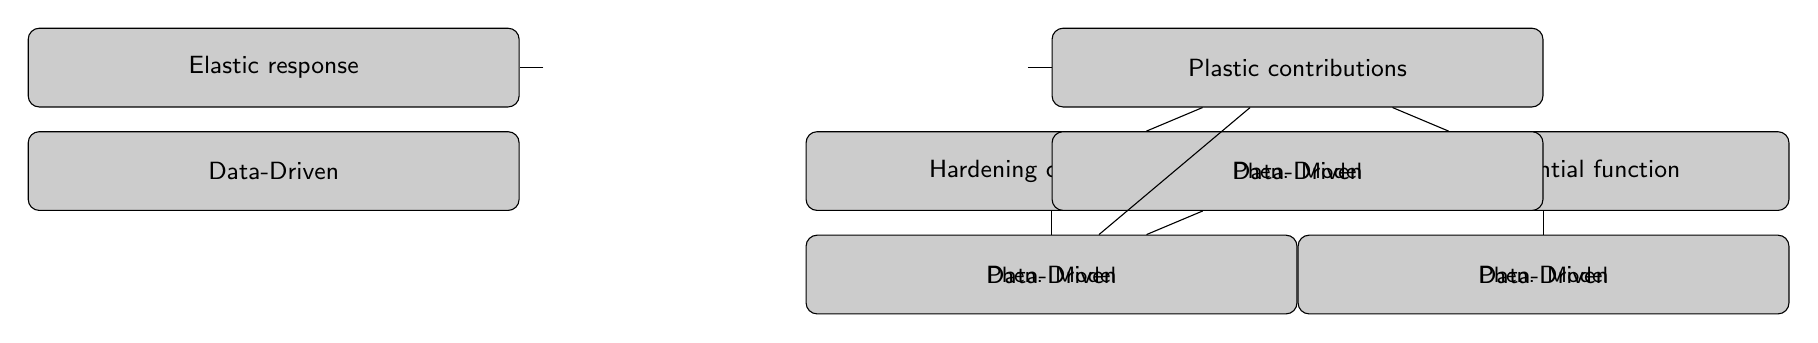
\begin{tikzpicture}[node distance=3mm]
\node[block, label={[label distance=3mm,xshift=-0.75cm,yshift=0cm,yshift=-0.3cm,rotate=0]90:Elastoplasticity}] (ElasPlasticity) {};
\node[block,left=of ElasPlasticity] (Elastic) {Elastic response};
\node[block,right=of ElasPlasticity] (Plastic) {Plastic contributions};
\node[block,below=of Elastic] (DD) {Data-Driven};
\node[block,below=of Plastic,anchor=north west] (Potential) {Yield / potential function};
\node[block,below=of Plastic,anchor=north east] (Harden) {Hardening components};
\node[block,below=of Potential] (DDPot) {Data-Driven};
\node[block,below=of Plastic] (DDHarden) {Data-Driven};
\node[block,below=of Harden] (DDFlow) {Data-Driven};
\node[block,below=of Potential,label={[label distance=3mm,xshift=0.25cm,yshift=0cm,yshift=-0.3cm,rotate=0]90:Phen. Model}] (DDPotPhenModel) {Phen. Model};
\node[block,below=of Plastic,label={[label distance=3mm,xshift=0.25cm,yshift=0cm,yshift=-0.3cm,rotate=0]90:Phen. Model}] (DDFlowPhenModel) {Phen. Model};
\node[block,below=of Harden,label={[label distance=3mm,xshift=0.25cm,yshift=0cm,yshift=-0.3cm,rotate=0]90:Phen. Model}] (DDHardenPhenModel) {Phen. Model};
\draw (ElasPlasticity)--(Elastic);
\draw (ElasPlasticity)--(Plastic);
\draw (Plastic)--(Potential);
\draw (Plastic)--(Harden);
\draw (Plastic)--(DDFlow);
\draw (Potential)--(DDPotPhenModel);
\draw (Potential)--(DDPot);
\draw (Harden)--(DDHardenPhenModel);
\draw (Harden)--(DDHarden);
\draw (DDFlow)--(DDFlowPhenModel);
\end{tikzpicture}
\end{document}